\documentclass{article}
\usepackage[utf8]{inputenc}
\usepackage[spanish]{babel}

% Formato de página
\usepackage[letterpaper, margin = 1.5cm]{geometry}

% Más opciones para enumerar
\usepackage{enumitem}

% Manejo de imágenes
\usepackage{graphicx}
\usepackage{wrapfig}
\graphicspath{{img/}}
\usepackage{float}

\begin{document}
    \title{
        Fundamentos de bases de datos \\
        Tarea 3 \\
        Modelo Relacional
    }
    \author{
        Díaz Gómez Silvia \\
        Eugenio Aceves Narciso Isaac \\
        Quiroz Castañeda Edgar
    }
    \date {
        22 de marzo del 2019    
    }
    \maketitle

    \section{Preguntas de repaso}
    \begin{enumerate}[label = \alph*.]
        \item ¿Qué es una \textbf{relación} y qué características tiene?
        \item ¿Qué es un \textbf{esquema de relación}?
        \item ¿Qué es una \textbf{llave primaria} ¿qué es una \textbf{llave 
        candidata}? ¿qué es una \textbf{llave mínima}? ¿qué es una \textbf{super
        llave}
        \item ¿Qué restricciones impone una \textbf{llave primaria} y una llave 
        foránea al modelo de dato relacional?
        \item Investiga cómo se traducen las \textbf{categorías} (presentes en
        el \textbf{modelos E/R}) al \textbf{modelos relacional}. Proporciona un 
        ejemplo.
    \end{enumerate}

    \section{Modelo relacional}
    Traduce el siguiente modelo \textbf{Entidad/Relación} a su correspondiente 
    \textbf{Modelo Relacional}:
    
    \begin{center}
        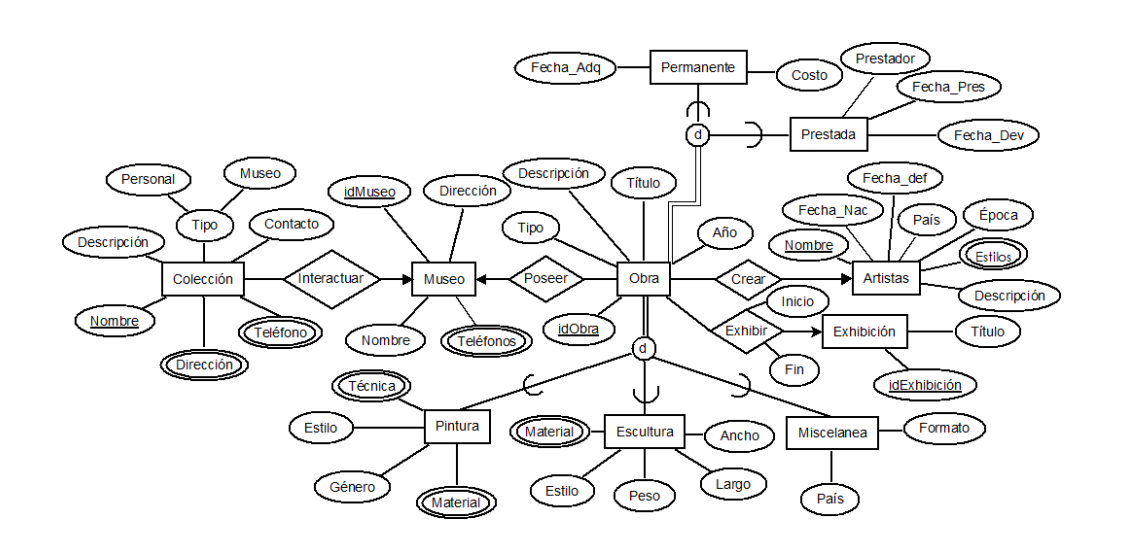
\includegraphics[width=1\textwidth]{er1.png}
    \end{center}

    \begin{figure}[H]
    	\begin{center}
    		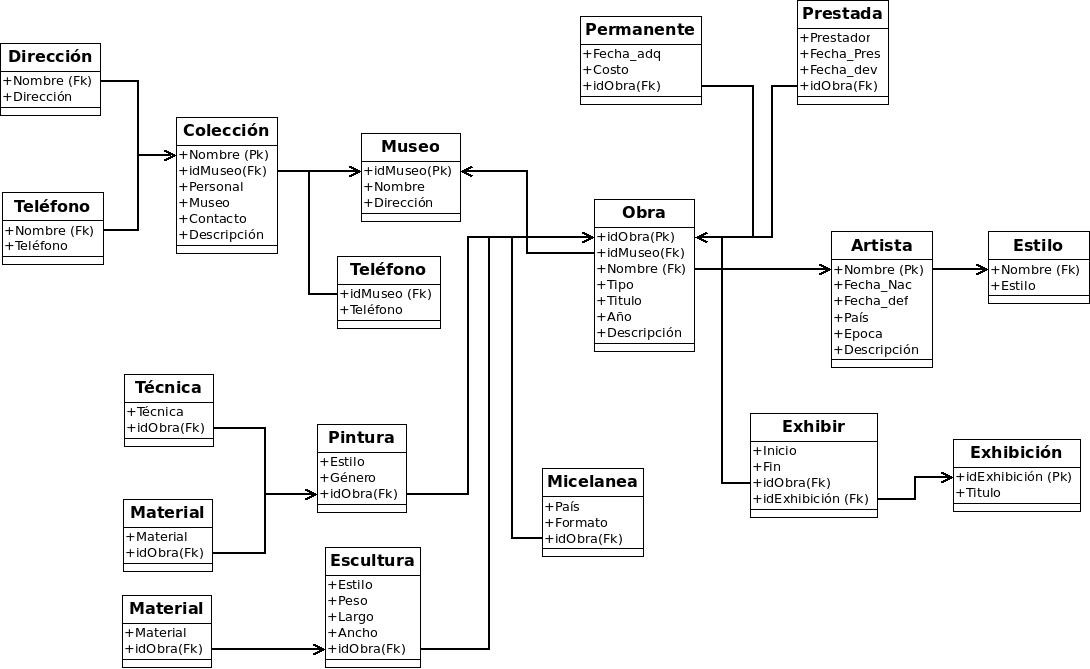
\includegraphics[width=1\textwidth]{MRProblema2.jpeg}
    	\end{center}
    	\caption{Traducción del modelo E-R de la figura anterior al modelo Relacional.}
    \end{figure}
        
    \section{Modelo relacional}
    Traduce s su correspondiente \textbf{Modelo Relacional} el problema del 
    \textbf{Sistema de Información Geográfica (Tarea 1)}. Se realizaste alguna
    modificación a tu diseño orignal (para mejorarlo) indica los cambios hechos 
    y la justificación de los mismos.\\
    En cualquier caso, deberás mostrar el \textbf{diagrama E/R} y su
    correspondiente traducción. Es importante que muetres tanto las 
    \textbf{restricciones de entidad} como las de \textbf{integridad referencial}.
    
    \begin{figure}[H]
    	\begin{center}
    		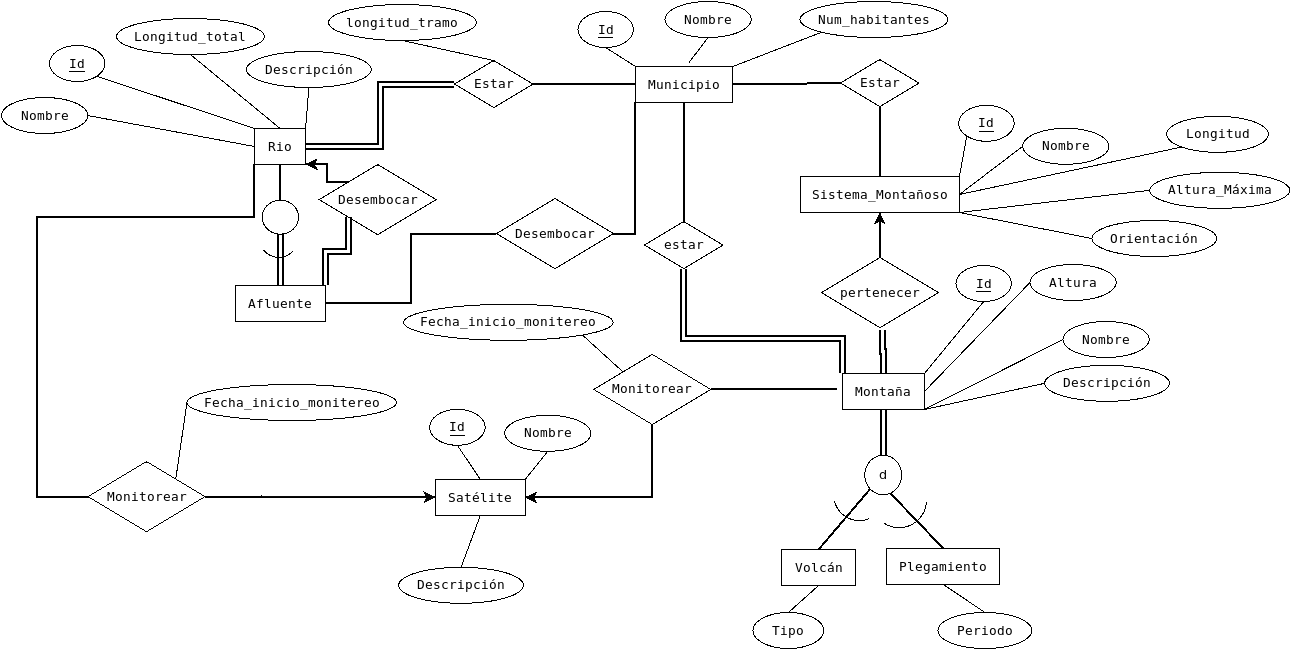
\includegraphics[width=1\textwidth]{2b.png}
    	\end{center}
    	\caption{Modelo E-R para el Sistema de Información Geográfica.}
    \end{figure}
    
    \begin{figure}[H]
      \begin{center}
      	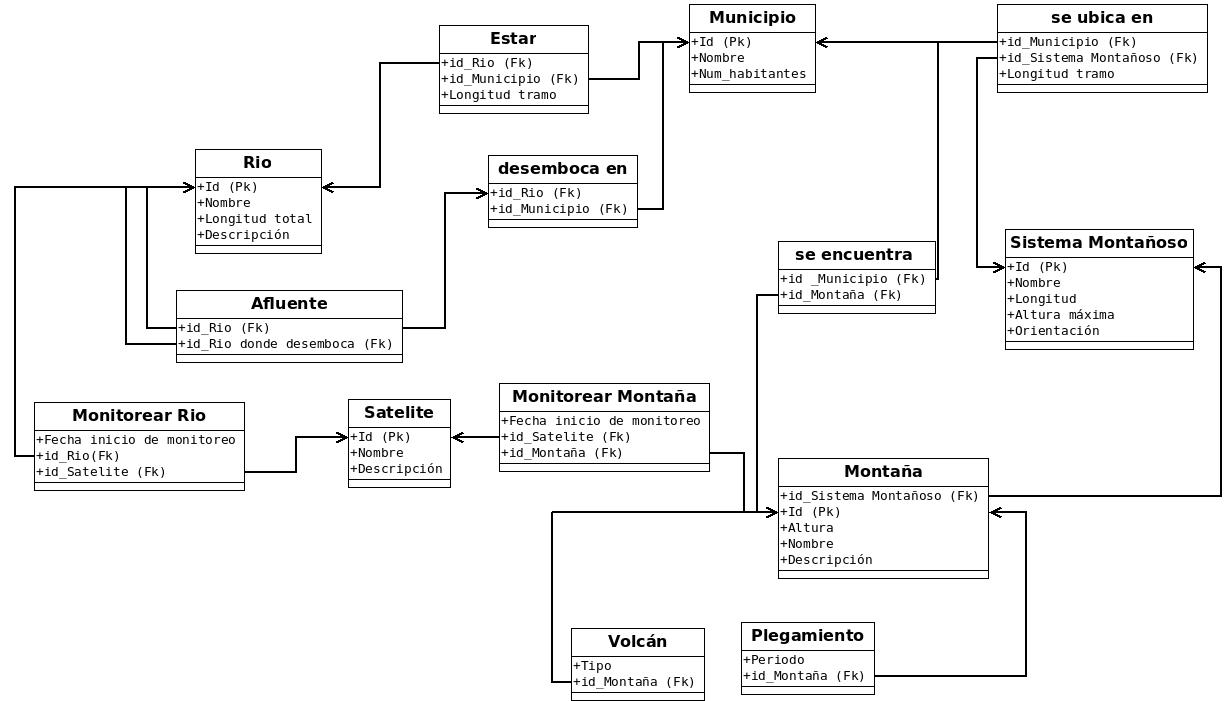
\includegraphics[width=1\textwidth]{esquemaRelacionalGeo.jpeg}
      \end{center}
      \caption{Traducción del modelo E-R para el Sistema de Información Geográfica a  Esquema Relacional.}
   \end{figure}

    \section{Lectura}
    Leer el artícula \textbf{Codd's 12 Rules for a RDBMS}. Explica con tus 
    propias palabras cada una de las 12 reglas de \textbf{Codd}.\\
    Indica por qué consideras que son importantes y si, hasta el momento de lo 
    comentado en el curso, sería posible que un \textbf{SMBD} pudiera cumplir 
    enteramente con lo que ahí se propone.
    
    \begin{itemize}
    	\item\textbf{Regla 1 : The Information Rule}\\
        Toda la información debe estar representada en el esquema lógico de la 
        base de datos. Y debe estar represetada como entradas de una tabla.\\
        Si los datos no están en el esquema lógico, entonces no sería accesibles
        usando los mecanismos de consulta del sistema, por lo que es como si 
        los datos no estuvieran ahí.\\
        Esto se puede lograr en SMBD forzando a que la única manera de almacenar 
        datos sea a través de inserciones en tablas.
    	\item\textbf{Regla 2 : Guaranteed Access Rule}
        Toda la información debe ser accesible. Esto es que todo dato tenga un 
        identificador o llave primaria, además de  que los datos sean atomicos 
        ya que son de suma importancia para poder garantizar la accesibilidad a 
        los datos.\\
        Esto es importante porque no poder acceder a los datos es equivalente a
        no tener los datos. \\
        Sería posible que un SMBD pueda garantizar esto si a todos los datos 
        insertdos bien se les exige una llave al momento o se les asigna un 
        llave sintética al ser ingresados.\\
        Aunque forzar lo segundo podría llevar bien a redundancia o que ya no 
        se refleje totalmente el esquema lógico de la base de datos.
    	\item\textbf{Regla 3: Systematic Treatment of NULL Values}\\
        Debe existir un valor NULL diferente de todos los demás posibles datos 
        que represente la ausencia de información y éste debe ser tratado de la 
        misma manera que todos los demás datos por el sistema.\\
        Esto es importante porque en otro caso no se podría represetar la 
        ausencia de información.\\
        Esto se puede lograr en un SMBD simplemente añadiendo el caso de NULL 
        como dato.
    	\item\textbf{Regla 4: Dynamic Online Catalog Based on the Relational Model}\\
        La estructura de la base de dato debe estar almacenada de igual manera 
        que el resto de los datos, para que pueda ser accesidad por usuarios usando
        los mecanismos ordinarios de consulta.\\
        Esto puede ser importante para desarrollar aplicaciones que utilicen la 
        base de datos, aunque no tanto para el usuario de esas aplicaciones.\\
        Esto se es posible en un SMBD teninendo tablas administrativas sobre 
        el resto de las tablas dentro de la misma base de datos.
    	\item\textbf{Regla 5: Comprehensive Data Sublanguage Rule}\\
        Se debe tener soporte para algún lenguaje formal que permita definir tipos
        de datos, hacer consultas, transacciones, y definir restricciones.\\
        Esto es necesario para facilitar la automatización y manejo avanzado de
        la base de datos, aunque si se tiene otro mecanismo que no es un lenguaje
        pero que realiza todo lo necesario, sería suficiente para manejar la base
        de datos, aunque puede alenter o provocar problemas al intentar 
        manipulaciones muy específicas.\\
        En general, en una SMBD esto se logra con un dialecto de SQL.
    	\item\textbf{Regla 6: View Updating Rule}\\
        Todas las vistas que son teóricamente actualizables deben de poder ser 
        actualizadas.\\
        Esto es importante porque aunque algo sea teóricamente posible, si no se 
        factible su ejecución, para fines prácticos es imposible.
    	\item\textbf{Regla 7: High-Level Insert, Update, and Delete}\\
        Las operaciones de modificación de la base de datos deben estar 
        disponilbes en términos de conjuntos de tuplas, no de tuplas
        individuales.\\
        Esto haría más eficiente las transacciones con grandes cantidades de 
        datos. Su ausencia sólo haría más lento todo, por lo que no es tan
        indispensable.\\
        Esto se pude lograr implementando todas las operaciones de la base de
        datos en términos de conjuntos directamente, por lo que sería posible
        que un SMBD tenga esta característica.
    	\item\textbf{Regla 8: Physical Data Independence}\\
        Esta regla menciona que a nivel fisico que es donde la base de datos 
        almacena e implementa los metodos de acceso a los datos es independiente 
        de la manera lógica en que se accede, por lo tanto los cambios que se 
        hagan a nivel físico no le afecta al usuario puesto que al usuario no le 
        interesa saber como se almacena o como se acceden a los datos. \\
        Es importante porque permite que los usuarios y los desarrolladores no
        tengan que lidiar con problemas físicos de la base de datos, y también
        que los encargados de la parte física no tengan que concer la estructura
        ni los problemas lógicos de la base de datos.\\
        De cualquier manera, en algún punto tiene que haber contacto entre los 
        niveles lógico y físico para acceder a la información, así que siempre
        va a exisitir alguna situación donde un problema físico afecte al esquema
        lógico.
    	\item\textbf{Regla 9: Logical Data Independence}\\
        El esquema de la base de datos debe ser independiente de las aplicaciones
        que utilizan la base de datos. Esto es que se pueda modificar la estrucutura
        lógica de la base de datos sin necesidad de modificar las aplicaciones que
        la utilizan.\\
        Al igual que en el caso anterior, esto permite modularizar los problemas
        y responsabilidades.\\
        Y también como arriba, es imposible garantizarlo en todos los casos.
    	\item\textbf{Regla 10: Integrity Independence}\\
        Las restricciones de integridad deben de ser independientes del 
        funcionamiento de aplicaciones. Esto es que esas restricciones se puedan
        modificar sin necesidad de modificar las aplicaciones que utilizan la 
        base de datos. \\
        Igual en que las dos reglas anteriores, esto permite modularizar los
        problemas y responsabilidades. Pero como en algún momento las diferentes
        partes tienen que interactuar, es imposible garantizar que en todos los 
        casos se matiene la independencia.
    	\item\textbf{Regla 11: Distribution Independence}\\
        Una base de datos distribuida debe ser idéntica a una no distribuida 
        desde el punto de vista del usuario.\\
        Igual en que las reglas anteriores, esto permite modularizar las
        responsabilidades de cada parte. Pero como en algún momento hay un 
        proceso (cuyas circumstancias pueden ser impredecibles) de 
        división/recuperación de datos, entonces es imposible garantizar que en 
        todos los casos se mantiene.
    	\item\textbf{Regla 12: Non-Subversion Rule}\\
        Indica que no debe existir un mecasnimo para violar las restricciones.
        Es decir, en caso de que se propocione acceso de bajo nivel al sistema, 
        esta interfaz no debe ser capaz de modificar sin restricciones.\\
        Esto es importante porque si se pueden violar las restricciones, entonces 
        es como si o hubiera ninguna restricción.\\
        Esto se podría garantizar negando acceso de bajo nivel a la base datos,
        por lo que es posible que un SMBD lo tenga como característica.
    \end{itemize}
\end{document}